\documentclass{article}
\usepackage{bm}
\usepackage{amsmath}
\usepackage{graphicx}
\usepackage[left=25mm,right=25mm,top=25mm,bottom=25mm,paper=a4paper]{geometry}


\graphicspath{ {C:\Users\qwert\OneDrive\Documents\GitHub\ThreeBodyProblemVis\Images\averages1to100.png}}
\author{Caedan Miller, Kiki Murphy, Will St. John}
\title{MATH 312 Final Project Paper}

\begin{document}
\maketitle
\tableofcontents
\newpage
\section{Project Overview}
\subsection{Introduction}
The three body problem describes the problem of finding the positions of three objects with individual masses, initial positions, and initial velocities using Newtonian laws of motion and gravity. Unlike two body problems, closed-form solutions do not exist for the three body problem. In our case, this means that the positions of the three bodies must be approximated using numerical methods. In this paper, we will explore numerical solutions to the three body problem in two dimensions using Heun's Method. We will also explore the three body problem in two dimensions with the addition of masses and the gravitational constant $G$.


\subsection{Equations}
Newton's law of universal gravitation states that the gravitational force between two objects is proportional to the product of their masses and inversely proportional to the square of the distance between them. For object one in our system, this can be expressed mathematically as follows:
\begin{equation}
    \bm{F_{g,1}} = -G\frac{m_1 m_2}{|\bm{r_{12}}|^2}\bm{\hat{r_{21}}} -G\frac{m_1 m_3}{|\bm{r_{13}}|^2}\bm{\hat{r_{31}}}
\end{equation}
where $\bm{F_g}$ is the gravitational force between two objects, $G$ is the gravitational constant, $m_1$ and $m_2$ are the masses of the two objects, and $\bm{r}$ is the distance between the two objects.

The positional vector from one object to the next can be described as the difference in position vectors for the two objects. In other words:
\begin{equation}
    \bm{r_{12}} = \bm{r_1} - \bm{r_2}
\end{equation}

Additionally, the unit vector $\bm{\hat{r}}$ can be expressed as the positional vector divided by its magnitude.
\begin{equation}
    \bm{\hat{r}} = \frac{\bm{r}}{|\bm{r}|}
\end{equation}

Using equations (2) and (3), equation (1) can be rewritten as follows:

\begin{equation}
    \bm{F_{g,1}} = -Gm_1 m_2\frac{\bm{r_1} - \bm{r_2}}{|\bm{r_1} - \bm{r_2}|^3}-Gm_1 m_3\frac{\bm{r_1} - \bm{r_3}}{|\bm{r_1} - \bm{r_3}|^3}
\end{equation}


Newton's second law of motion states that the acceleration of an object is proportional to the net force acting on it and inversely proportional to its mass. This can be expressed mathematically as follows:
\begin{equation}
    \bm{F_{net}} = m\bm{a}
\end{equation}
where $F_{net}$ is the net force acting on an object, $m$ is the mass of the object, and $a$ is the acceleration of the object.

Setting equation (5) with $m=m_1$ equal to equation (4) and solving for acceleration yields the following relationship for the acceleration of object one:

\begin{align}
    \bm{F_{net,1}} &= \bm{F_{g,1}} \nonumber \\
    m_1\bm{a_1} &= -Gm_1 m_2\frac{\bm{r_1} - \bm{r_2}}{|\bm{r_1} - \bm{r_2}|^3}-Gm_1 m_3\frac{\bm{r_1} - \bm{r_3}}{|\bm{r_1} - \bm{r_3}|^3}\nonumber \\
    \bm{a_1} &= -Gm_2\frac{\bm{r_1} - \bm{r_2}}{|\bm{r_1} - \bm{r_2}|^3}-Gm_3\frac{\bm{r_1} - \bm{r_3}}{|\bm{r_1} - \bm{r_3}|^3}
\end{align}

Similar equations can be found for the other two objects in the system.  The result are three second-order differential equations can model the three body problem as described by Newtonian mechanics. These equations are as follows:

\begin{align}
    \ddot{\bm{r_1}} &= -Gm_2\frac{\bm{r_1}-\bm{r_2}}{|\bm{r_1}-\bm{r_2}|^3}-Gm_3\frac{\bm{r_1}-\bm{r_3}}{|\bm{r_1}-\bm{r_3}|^3}\\
    \ddot{\bm{r_2}} &= -Gm_1\frac{\bm{r_2}-\bm{r_1}}{|\bm{r_2}-\bm{r_1}|^3}-Gm_3\frac{\bm{r_2}-\bm{r_3}}{|\bm{r_2}-\bm{r_3}|^3}\\
    \ddot{\bm{r_1}} &= -Gm_1\frac{\bm{r_3}-\bm{r_1}}{|\bm{r_3}-\bm{r_1}|^3}-Gm_2\frac{\bm{r_3}-\bm{r_2}}{|\bm{r_3}-\bm{r_2}|^3}
\end{align}

where $r_1$, $r_2$, and $r_3$ are the vector positions of the three bodies, $m_1$, $m_2$, and $m_3$ are the masses of the three bodies, and $G$ is the gravitational constant.

\subsection{Simplification}

To simplify these three complicated equations, we limited the motion to only two dimensions instead of three. This allowed us to rewrite the equations as a system of six equations: three equations that describe the motion for each body only in the x direction, and three similar equations for the y direction. 
Equations (1), (2), and (3) can be rewritten as follows:
\begin{align}
    \ddot{r_1} &= -\frac{r_1-r_2}{|r_1-r_2|^3}-\frac{r_1-r_3}{|r_1-r_3|^3}\\
    \ddot{r_2} &= -\frac{r_2-r_1}{|r_2-r_1|^3}-\frac{r_2-r_3}{|r_2-r_3|^3}\\
    \ddot{r_3} &= -\frac{r_3-r_1}{|r_3-r_1|^3}-\frac{r_3-r_2}{|r_3-r_2|^3}
\end{align}
While these equations are already much more reasonable to work with, three body systems are still incredibly unstable with the added dependence on the mass ratio between the bodies, which influences the motion and can prevent symmetry within the problem. In addition, the gravitational constant that is used in astronomy is such a small number that we have to scale everything up so that there is still an attractive force between the bodies strong enough to influence each other. Because of this, we simplified these six motion equations even further by taking the mass of each body to be 1, and used a gravitational constant of 1. 
\begin{itemize}
    \item The three bodies only move in two dimensions.
    \item The three bodies are of equal mass $m_1 = m_2 = m_3 = 1$.
    \item The gravitational constant $G = 1$.
\end{itemize}

\subsection{Goals}
Our intended goal was to model the three body problem in the 2D plane for a range of initial conditions using Heun's Method. Once every approximation is complete, we would create a “moment map” of the result by averaging the amount of times a planet appears at a particular pixel and giving that pixel a corresponding RGB value. For example, a pixel where planet 1 (red) passes through numerous times would appear very dark red in the moment map, while a pixel where planet 1 (red) and 3 (blue) pass through a lot would appear purple.The steps towards this goal fall into two categories: those that we are certain we can achieve and those that are more ambitious.


The minimum viable product (MVP) of our project entails (1) rewritten equations for the three-body problem in two dimensions, (2) code in python to compute Heun's equations for all 12 of the three-body equations, and (3) plots of three-body motion featuring all three bodies and the center of mass in Python. 

\section{Process}
Our more ambitious goals entail the creation of the RGB map synthesizing the motion of the three bodies over a variety of initial conditions in order to achieve a better understanding of how the bodies tend to move. 
\subsection{Code}
\subsubsection{Necessary Packages}
\begin{verbatim}
import pandas as pd
import matplotlib.pyplot as plt
import numpy as np
import random
\end{verbatim}

\subsubsection{Heun's Method}
To rewrite Heun's Method in Python for this system of twelve differential equations, and ultimately solve for x and y position values for each body, we used what we know of simple Newtonian physics. We recognized that the equations we wrote for the three body problem in two dimensions were acceleration equations because they were time independent. To find the respective velocity and position, we only needed to take the first and second derivatives of the acceleration equations with respect to time.
We applied this to Heun's Method in one dimension by writing two functions - a Heun's Method function, and a derivative function - and finding the resulting vector of positions and velocities of all the bodies after each step. The Heun's Method function takes in a 12 dimensional p0 array that contains the initial positions and velocities for all bodies, and sets up a Dataframe to collect the position, velocity, and acceleration values of each after each step. For each step, the function calculates the derivative of the vector using the derivative function, and finds values for ptemp and the derivative of ptemp. It then reassigns the p0 vector to include the new values for position and velocity. The function also adds this data to a Dataframe so we can access the position, velocity, and acceleration points for each iteration.

\begin{verbatim}
def heun(p0: np.array, N: int, t: float) -> np.array:
    """Calculatue heuns method for the three body problem for N steps with step size t.

    Args:
        p0 (np.array): 12 dimensional vector of initial conditions corresponding to the following:
            p0[0] = x1, p0[1] = x2, p0[2] = x3, p0[3] = y1, p0[4] = y2, p0[5] = y3, 
            p0[6] = vx1, p0[7] = vx2, p0[8] = vx3, p0[9] = vy1, p0[10] = vy2, p0[11] = vy3
        N (int): number of steps
        t (float): step size

    Returns:
        np.array: np.array positions and velocities for each x and y of each planet
    """
    data = [p0[0], p0[1], p0[2], p0[3], p0[4], p0[5], 
            p0[6], p0[7], p0[8], p0[9], p0[10], p0[11], 
            derivative(p0)[6], derivative(p0)[7], derivative(p0)[8], 
            derivative(p0)[9], derivative(p0)[10], derivative(p0)[11]]
    df = pd.DataFrame(data=[data], columns=['P1: X Position', 'P2: X Position', 
                                'P3: X Position', 'P1: Y Position', 'P2: Y Position', 
                                'P3: Y Position', 'P1: X Velocity', 'P2: X Velocity', 
                                'P3: X Velocity', 'P1: Y Velocity', 'P2: Y Velocity', 
                                'P3: Y Velocity', 'P1: X Acceleration', 'P2: X Acceleration', 
                                'P3: X Acceleration', 'P1: Y Acceleration', 'P2: Y Acceleration', 
                                'P3: Y Acceleration'])

    for i in range(0, N):
        ptemp = p0 + t * derivative(p0)
        dp0 = derivative(p0)
        dptemp = derivative(ptemp)
        p0 = p0 + t/2 * (dp0 + dptemp)
        data = [p0[0], p0[1], p0[2], p0[3], p0[4], p0[5], p0[6], p0[7], p0[8], p0[9], p0[10], p0[11], 
            derivative(p0)[6], derivative(p0)[7], derivative(p0)[8], derivative(p0)[9], derivative(p0)[10], 
            derivative(p0)[11]]
        df2 = pd.DataFrame(data=[data], columns=['P1: X Position', 'P2: X Position', 
                                'P3: X Position', 'P1: Y Position', 'P2: Y Position', 
                                'P3: Y Position', 'P1: X Velocity', 'P2: X Velocity', 
                                'P3: X Velocity', 'P1: Y Velocity', 'P2: Y Velocity', 
                                'P3: Y Velocity', 'P1: X Acceleration', 'P2: X Acceleration', 
                                'P3: X Acceleration', 'P1: Y Acceleration', 'P2: Y Acceleration', 
                                'P3: Y Acceleration'])
        df2['P1: X Position'] = p0[0]
        df2['P2: X Position'] = p0[1]
        df2['P3: X Position'] = p0[2]
        df2['P1: Y Position'] = p0[3]
        df2['P2: Y Position'] = p0[4]
        df2['P3: Y Position'] = p0[5]
        df2['P1: X Velocity'] = p0[6]
        df2['P2: X Velocity'] = p0[7]
        df2['P3: X Velocity'] = p0[8]
        df2['P1: Y Velocity'] = p0[9]
        df2['P2: Y Velocity'] = p0[10]
        df2['P3: Y Velocity'] = p0[11]
        df = pd.concat([df, df2], ignore_index=True)
    
    df.insert(0, 'Time', [i * t for i in range(0, N + 1)])
    return df
\end{verbatim}

\subsubsection{Derivative}
While the Heun’s Method function is ultimately what allows us to model the three body problem with position and velocity points, the derivative function is just as important for the physics of the system. This function takes in the same 12 dimensional p0 vector that Heun’s Method does and it creates a new 12 dimensional p1 vector of the velocities and accelerations. Since the velocity values are already a part of the p0 vector, the derivative only reassigns those same values to the p1 vector. To find the accelerations for each body we use the rewritten time-independent three body equations, using the position values from the p0 vector. The derivative function then returns the p1 vector that we can use in Heun’s Method. 

\begin{verbatim}
def derivative(p0: np.array) -> np.array:
    """Calculates the derivative of the 12 dimensional vector p0.

    Args:
        p0 (np.array): 12 dimensional vecotr of initial conditions corresponding to the following:
            p0[0] = x1, p0[1] = x2, p0[2] = x3, p0[3] = y1, p0[4] = y2, p0[5] = y3, 
            p0[6] = vx1, p0[7] = vx2, p0[8] = vx3, p0[9] = vy1, p0[10] = vy2, p0[11] = vy3 

    Returns:
        np.array: 12 dimensional vector of the derivative of p0
    """
    p1 = 0 * p0
    p1[0] = p0[6]
    p1[1] = p0[7]
    p1[2] = p0[8]
    p1[3] = p0[9]
    p1[4] = p0[10]
    p1[5] = p0[11]
    p1[6] = - ((p0[0] - p0[1])/((p0[0]-p0[1])**2+(p0[3]-p0[4])**2)**(3/2)) - ((p0[0] - p0[2])/((p0[0]-p0[2])**2+(p0[3]-p0[5])**2)**(3/2))
    p1[7] = - ((p0[1] - p0[0])/((p0[1]-p0[0])**2+(p0[4]-p0[3])**2)**(3/2)) - ((p0[1] - p0[2])/((p0[1]-p0[2])**2+(p0[4]-p0[5])**2)**(3/2))
    p1[8] = - ((p0[2] - p0[0])/((p0[2]-p0[0])**2+(p0[5]-p0[3])**2)**(3/2)) - ((p0[2] - p0[1])/((p0[2]-p0[1])**2+(p0[5]-p0[4])**2)**(3/2))
    p1[9] = - ((p0[3] - p0[4])/((p0[0]-p0[1])**2+(p0[3]-p0[4])**2)**(3/2)) - ((p0[3] - p0[5])/((p0[0]-p0[2])**2+(p0[3]-p0[5])**2)**(3/2))
    p1[10] = - ((p0[4] - p0[3])/((p0[1]-p0[0])**2+(p0[4]-p0[3])**2)**(3/2)) - ((p0[4] - p0[5])/((p0[1]-p0[2])**2+(p0[4]-p0[5])**2)**(3/2))
    p1[11] = - ((p0[5] - p0[3])/((p0[2]-p0[0])**2+(p0[5]-p0[3])**2)**(3/2)) - ((p0[5] - p0[4])/((p0[2]-p0[1])**2+(p0[5]-p0[4])**2)**(3/2))
    return p1
\end{verbatim}
When we first started thinking through how we were going to solve Heun’s Method for these two systems of 12 equations, we were overwhelmed by how complicated this seemed. In our first attempts we tried to use Heun’s Method in two dimensions and then somehow solve for the extra variables what we knew about physics. Ultimately we didn’t get very far with this approach. The problem became much more simple when we started thinking of these 12 differential equations that seemed to all depend on each other as less of a system of equations and more as a set of independent points that made up one big vector. By changing our perspective, we were also able to incorporate what we know about Newtonian physics to relate the time-independent acceleration equations to the position and velocity values we cared about, something we were not able to do before. This also allowed us to simplify Heun’s Method to only depend on one variable instead of two, which both made the code shorter and made the three body problem easier to understand. 
\subsubsection{Perterbations}
\begin{verbatim}
def perterbations(N: int) -> list:
    """Randomly generates N positions within the first two quadrants of a circle 
        with radius less than or equal to 0.01.

    Args:
        N (int): number of positions to generate

    Returns:
        list: tuples of x and y positions
    """
    positions = []
    while len(positions) < N:
        x = random.randrange(-1000, 1000, 1) / 10000
        y = random.randrange(0, 1000, 1) / 10000
        if x**2 + y**2 <= 0.01:
            positions.append((x, y))
    return positions
\end{verbatim}

\subsubsection{Making Plots}
\begin{verbatim}
    def make_vis(pos: int, pert: int, title: str) -> None:
    """Creates a visualization of the three body problem with pert perturbations. Indended 
    to be used with subplots.

    Args:
        pos (int): subplot position for the visualization
        pert (int): number of perterbations to include in the plot
        title (str): title of the plot
    """
    mid_pos = perterbations(pert)

    p = np.array([-1, 1, 0, 0, 0, 0, 0, 0, 0, -1, 1, 0])
    d = heun(p, 5000, 0.001)
    plt.subplot(pos)

    plt.title(title)
    plt.plot(d['P1: X Position'][0], d['P1: Y Position'][0], c='red', marker='x', label='Earth')
    plt.plot(d['P2: X Position'][0], d['P2: Y Position'][0], c='green', marker='x',label='Mars')
    plt.plot(d['P3: X Position'][0], d['P3: Y Position'][0], c='blue', marker='x', label='Venus')
    plt.plot(d['P1: X Position'], d['P1: Y Position'], c='red', alpha=0.3, label='Earth')
    plt.plot(d['P2: X Position'], d['P2: Y Position'], c='green', alpha=0.3, label='Mars')
    plt.plot(d['P3: X Position'], d['P3: Y Position'], c='blue', alpha=0.3, label='Venus')

    for x, y in mid_pos:
        p = np.array([-1, 1, x, 0, 0, y, 0, 0, 0, -1, 1, 0])
        d = heun(p, 5000, 0.001)        
        plt.plot(d['P1: X Position'], d['P1: Y Position'], c='red', alpha=0.5)
        plt.plot(d['P2: X Position'], d['P2: Y Position'], c='green', alpha=0.5)
        plt.plot(d['P3: X Position'], d['P3: Y Position'], c='blue', alpha=0.5)
    return
\end{verbatim}

\subsubsection{Making Average Plots}
\begin{verbatim}
def generate_avg(pert: int, pos: int, duration: int, stepsize: float) -> None:
    """Creates an average of pert perterbations using Heun's method for a particular duration and stepsize.

    Args:
        pert (int): number of perterbations to plot
        duration (int): how many steps to take
        stepsize (float): step size for heun's method
    """
    x1 = []
    x2 = []
    x3 = []
    y1 = []
    y2 = []
    y3 = []
    mid_pos = perterbations(pert)
    plt.subplot(pos)

    for x, y in mid_pos:
            p = np.array([-1, 1, x, 0, 0, y, 0, 0, 0, -1, 1, 0])
            d = heun(p, duration, stepsize)
            x1.append(d['P1: X Position'])
            x2.append(d['P2: X Position'])
            x3.append(d['P3: X Position'])
            y1.append(d['P1: Y Position'])
            y2.append(d['P2: Y Position'])
            y3.append(d['P3: Y Position'])
            plt.plot(d['P1: X Position'], d['P1: Y Position'], c='red', alpha=0.1)
            plt.plot(d['P2: X Position'], d['P2: Y Position'], c='green', alpha=0.1)
            plt.plot(d['P3: X Position'], d['P3: Y Position'], c='blue', alpha=0.1)

    x1avg = np.mean(x1, axis=0)
    x2avg = np.mean(x2, axis=0)
    x3avg = np.mean(x3, axis=0)
    y1avg = np.mean(y1, axis=0)
    y2avg = np.mean(y2, axis=0)
    y3avg = np.mean(y3, axis=0)

    plt.title(f"Average of {pert} Perturbations")
    plt.plot(x1avg, y1avg, c='red', alpha=1)
    plt.plot(x2avg, y2avg, c='green', alpha=1)
    plt.plot(x3avg, y3avg, c='blue', alpha=1)
    return
\end{verbatim}

\subsection{Adding Masses \& G}
At one point, we wanted to better modify our simulations to account for the mass of the planets and the gravitational constant G. To do this, we added a vector of the three bodies' respective masses into the input for Heun’s method and the derivative functions and then incorporated the masses into the calculations within the functions. We were able to verify that this produced the same results as our original simplified code by executing it with masses of 1/G. After this, we then attempted to create more accurate simulations of astronomical phenomena, specifically the earth-moon-sun system of gravitational interactions. However, this was largely unsuccessful. With the earth-moon-sun system specifically, the distance between the earth and moon is small compared to the distance between the earth and the sun, and even if the relative masses are scaled down as far as possible, the sun is so much more massive than the moon that it was too difficult to produce any valuable plots with the code that we were using. 
	Additionally, the magnitude of G is so small that any realistic astronomical simulations would have to feature enormous masses and very long distances, two factors that not only make it very difficult to create readable plots but would force us to use more complicated initial velocities when modeling stable conditions. This led us to abandon the idea of accounting for mass and gravity within our main project and stick with our simplified three body problem. 

\subsection{Exploring Collinear Initial Conditions}
\begin{figure}[h!]
    \centering
    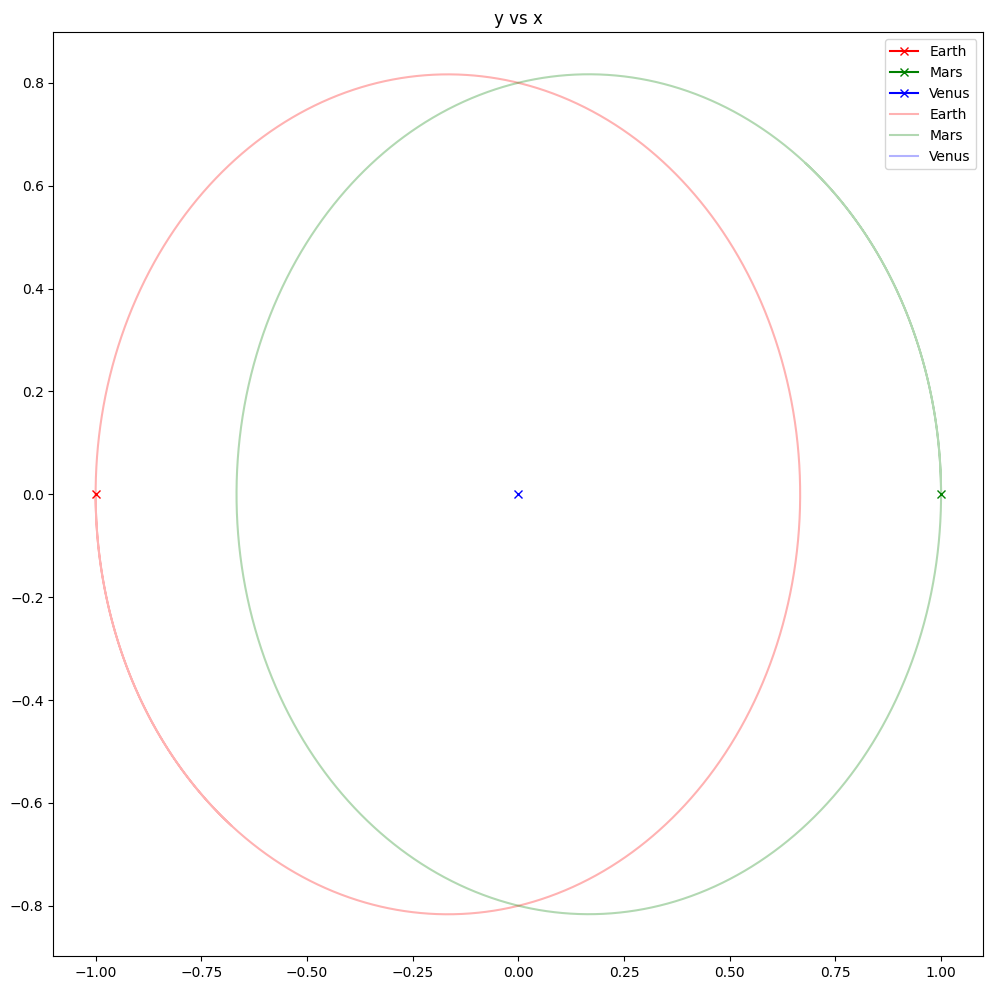
\includegraphics[width=0.8\textwidth]{Images/noPerterbations.png}
    \caption{Numerical solution to the three body problem with no perterbations.}
    \label{fig:mesh2}
\end{figure}

Three body systems are already prone to instability, so finding stable three body systems was difficult. In these cases, we discovered that the motion would tend to simplify in one of two ways. The first of these was that the three body system would almost immediately simplify to a two body system, with the third body orbiting the other two. In the other case, two of the three bodies would crash into each other, flinging both of them away from the rest of the system. 

We eventually found that collinear three body systems seemed to be the most stable and less likely to exhibit the behaviors we had noticed before. From looking at resources we were able to find examples of stable three body systems and replicate them in our own code. These examples all used equal masses of 1 and a gravitational constant of 1, and had the initial positions of each body set to (-1, 0), (0, 0), (1, 0), respectively. In these examples, none of the three bodies exhibited chaotic behavior.
In our modeling of the three body problem we used these same parameters, only changing the initial position of the center body slightly with each iteration to track how the system evolved. We selected these initial positions by writing code that randomly chose points within a sphere centered at the origin with radius 0.1. Since the collinear system we chose was symmetric, we were also able to simplify the code to only selected points from the top half of the sphere, knowing that the motion would be mirrored for initial positions chosen on the bottom half. 
\newpage
\section{Results and Discussion}
\begin{figure}[h!]
    \centering
    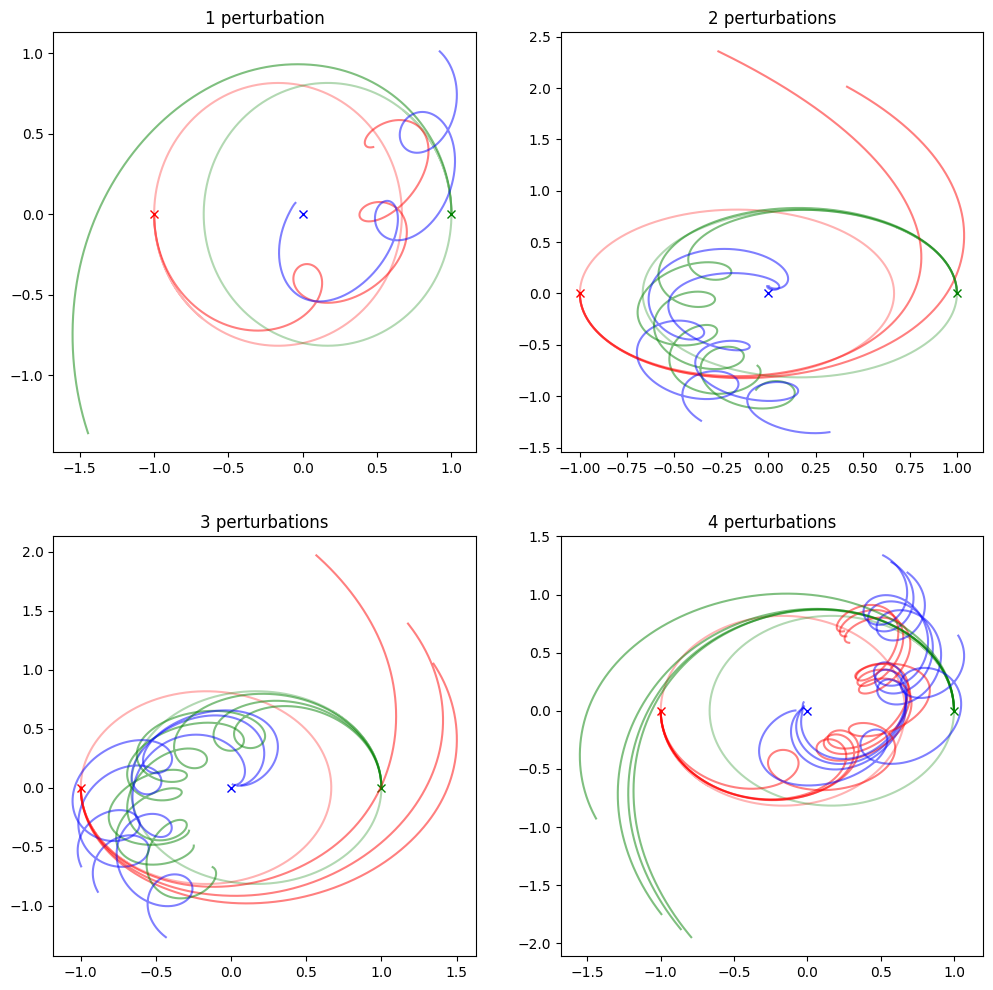
\includegraphics[width=0.8\textwidth]{Images/perterbations1to4.png}
    \caption{Numerical solution to the three body problem with a range of perturbations.}
\end{figure}

\newpage
\begin{figure}[h!]
    \centering
    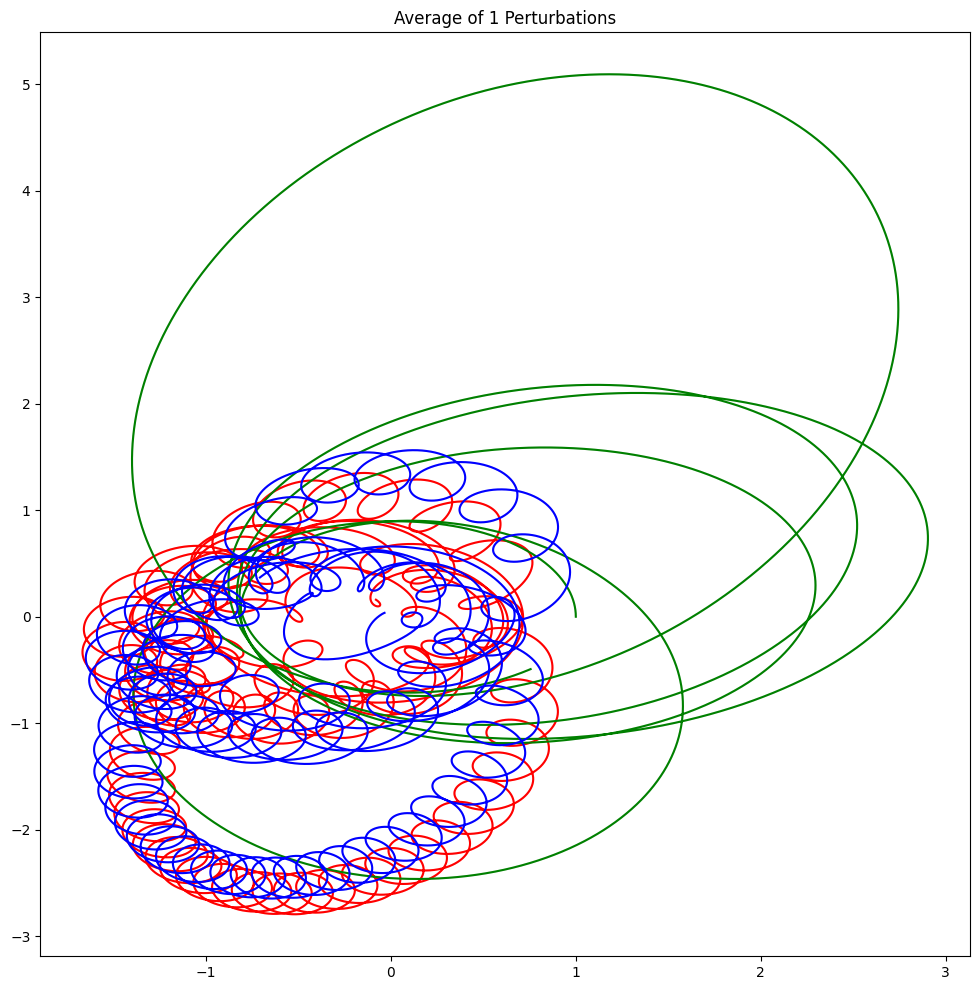
\includegraphics[width=0.8\textwidth]{Images/longrun.png}
    \caption{Numerical solution to the three body problem with a single perturbation, ran for approximately 20x as long.}
\end{figure}
\newpage
\begin{figure}[h!]
    \centering
    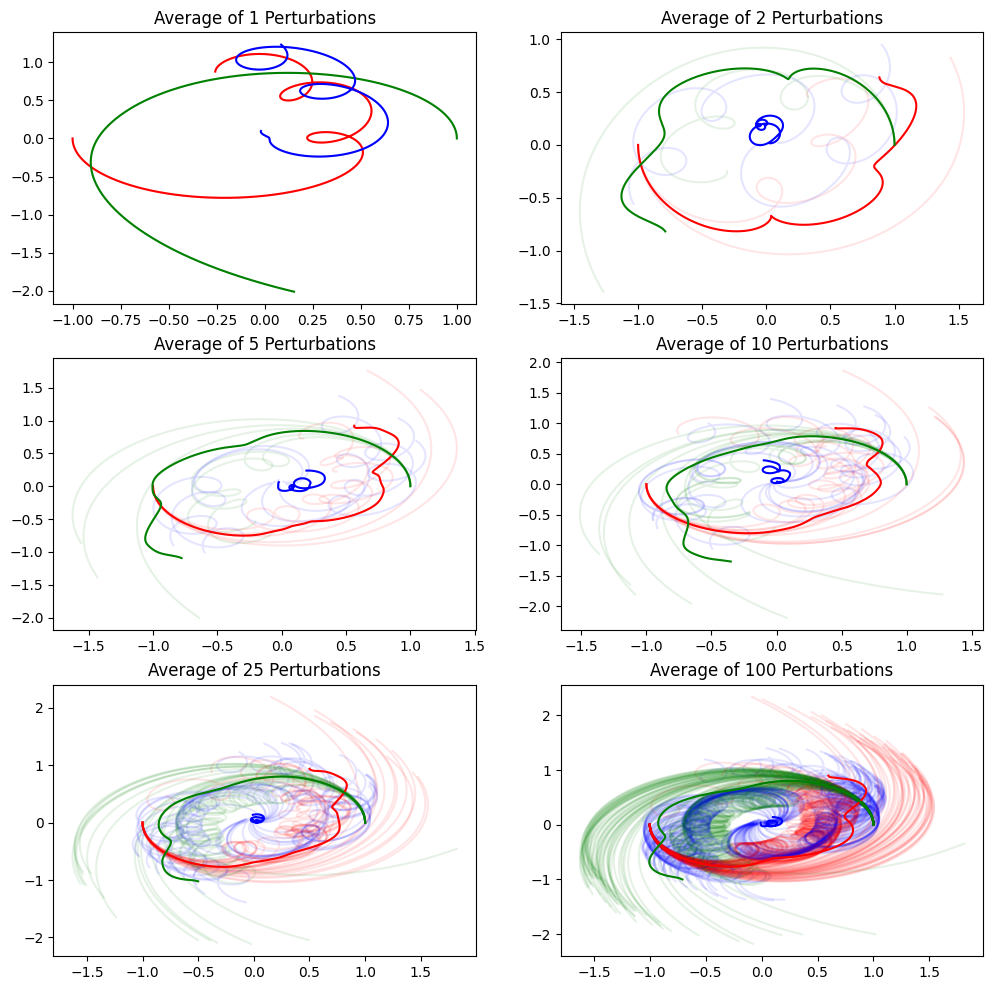
\includegraphics[width=0.8\textwidth]{Images/averages1to100.png}
    \caption{Numerical solution to the three body problem with 1 to 100 perturbations, averaged together.}
\end{figure}

Through many perturbations, we gleaned a variety of insights into the behavior of the three body problem under these collinear initial conditions. Firstly, the planet on whichever side is closest to the center planet will be attracted to the center planet and they will spiral around each other, while the third planet will rotate distantly around the other two. Within the shorter time period of most of our plots, it appears that the third planet accelerates off into space, but when we ran one perturbation for a very long time, the third planet remained within the picture the entire time. Thus, the long-term behavior does not indicate the loss of the third planet. 

\section{Conclusion}
Given our initial conditions, duration, and step size, we concluded that Huen's numerical approximation to the three body problem simplifies into a two body problem, where one body is comprised of two objects engaged in a "dance" about each other, while the other body interacts from a much larger distance.

Solutions also exhibit two forms of symmetry. The first is rotational quadrant symmetry, where the third and fourth quadrants are rotated images of the first and second. The second is local symmetry, where solutions with similar initial conditions in a particular quadrant follow similar paths.

\section{Limitations}
\subsection{Runtime}
The runtime of our plots is a function of the number of perturbations, the duration of the simulation and the stepsize. We estimated that creating a single plot of 50 perturbations takes approximately 30 minutes. If we could figure out a more effienct method for creating these plots, we could create more plots and explore more initial conditions.

\subsection{Stable Solutions}
A Three Body system is a chaotic system. We were limited by this fact as any initial condition we wanted to explore had to be stable. There are a limited number of initial conditions available, so we decided to improvise to save fime and explore collinear initial conditions. We would have like to be able to explore more stable initial conditions.

\subsection{Masses}
Our plots do not incorporate the masses of the three bodies. We would have liked to incorporate the masses, however, this adds another layer of uncertainty to our Stable Solution problem described above. Not only do the three bodies have to have stable intial positions and velocities, but now the masses of each body interact to a higher degree.

\subsection{Turtle Graphics}
One of our goals was to create a visualization of the three body problem using turtle graphics. We were able to achieve this, however, the turtle animation was slow, even at its highest setting.

\subsection{Astronomical Scale}
Another goal of our was to create a visualization of the three body problem on an astronomical scale. We were able to achieve this, however, the scale of the plot was so large that the three bodies were not visible. We would have liked to be able to zoom in on the three bodies, but this was not possible with the turtle graphics, nor our time constaint.

\end{document}